\newpage

\section{Problem 5.27}
\subsection{重要数据展示}
对于拟合函数
\[\phi(t,\bm{x})=(1-x_1t/x_2)^{(1/(x_1c)-1)}\]设$y_1=x_1/x_2,\quad y_2=1/(x_1c)$,则原函数变为:
\[\phi(t,\bm{y})=(1-ty_1)^{(y_2-1)}\]

那么残量$\bm{r(x)}=\phi(\bm{t},\bm{y})-\bm{d}$
,该问题为极小化函数
\begin{equation}
\text{minimize}\quad f(\bm{x})=\dfrac{1}{2}\bm{r(x)^Tr(x)}
\end{equation}

\subsection{算法伪代码}
\begin{algorithm}[h]  
\caption{Gauss-Newton method for problem(5.27)}  
\begin{algorithmic}[1]  
\STATE Given $\bm{y}^{(0)},k=0$ 
\STATE Set $\bm{r}^{(0)}=\phi(\bm{y}^{(0)})-\bm{d}$ 
\WHILE {$\|\bm{r}^{(k)}\|>\epsilon$}
\STATE Set $\bm{r}^{(k)}=\phi(\bm{y}^{(k)})-\bm{d}$
\STATE Set ${\bm{A}^{(k)}}^T=\nabla {\bm{r}^{(k)}}^T$
\STATE Set $\bm{s}^{(k)}=-({\bm{A}^{(k)}}^T{\bm{A}^{(k)}})^{-1}{\bm{A}^{(k)}}^T{\bm{r}^{(k)}}$
\STATE Compute $\alpha_k$ by Line Search(\textbf{Algorithm} \ref{Amj})
\STATE Set $\bm{y}_{k+1}=\bm{y}_{k}+\alpha_k\bm{s}^{(k)}$
\STATE Set $k=k+1$
\ENDWHILE
\RETURN $\bm{y}^{(k)}$ as $\bm{y}^{\star}$
\end{algorithmic}  
\end{algorithm}




\subsection{计算结果展示}
此题采用线搜索确定步长时,需要加入越界判定:检查函数点是否迭代出定义域外,如果是,则缩减步长。

其中,定义域需要满足$1-\bm{t}y_1>0$即可,取$\bm{t}$中最大值50000,那么只需满足$y_1<1/50000$即可。
\begin{lstlisting}
ak=1;
while(Check(y+ak*s))		%越界判定
		ak=0.5*ak;
end

function bool=Check(y)		%检查函数是否越界
    bool=(y(1)>=1/50000);
    return 
end
\end{lstlisting}

在这次编程实验中,参数的调节成为了一个非常重要的因素,无论是初值的选择、初始的步长选择、线搜索中的$\gamma$和$\rho$,都将极大地影响程序的运行结果,经过辛勤地调参,最后确定了以下参数,使得程序误差较小。

此次我编写了两个GN程序,一个是带线搜索的,其中$\gamma=0.6,\rho=0.5$,初始点为$(-1,-2)$,另一个是不带线搜索的,其中确定步长$\alpha_k=0.05$,初始点为$(-1,10)$。

残量的2-范数随迭代次数的下降情况如下:(由于数量级巨大,为了更好的显示残差的波动,将原图中将残差取对数处理后并排参考)

\begin{figure}[H]
\centering
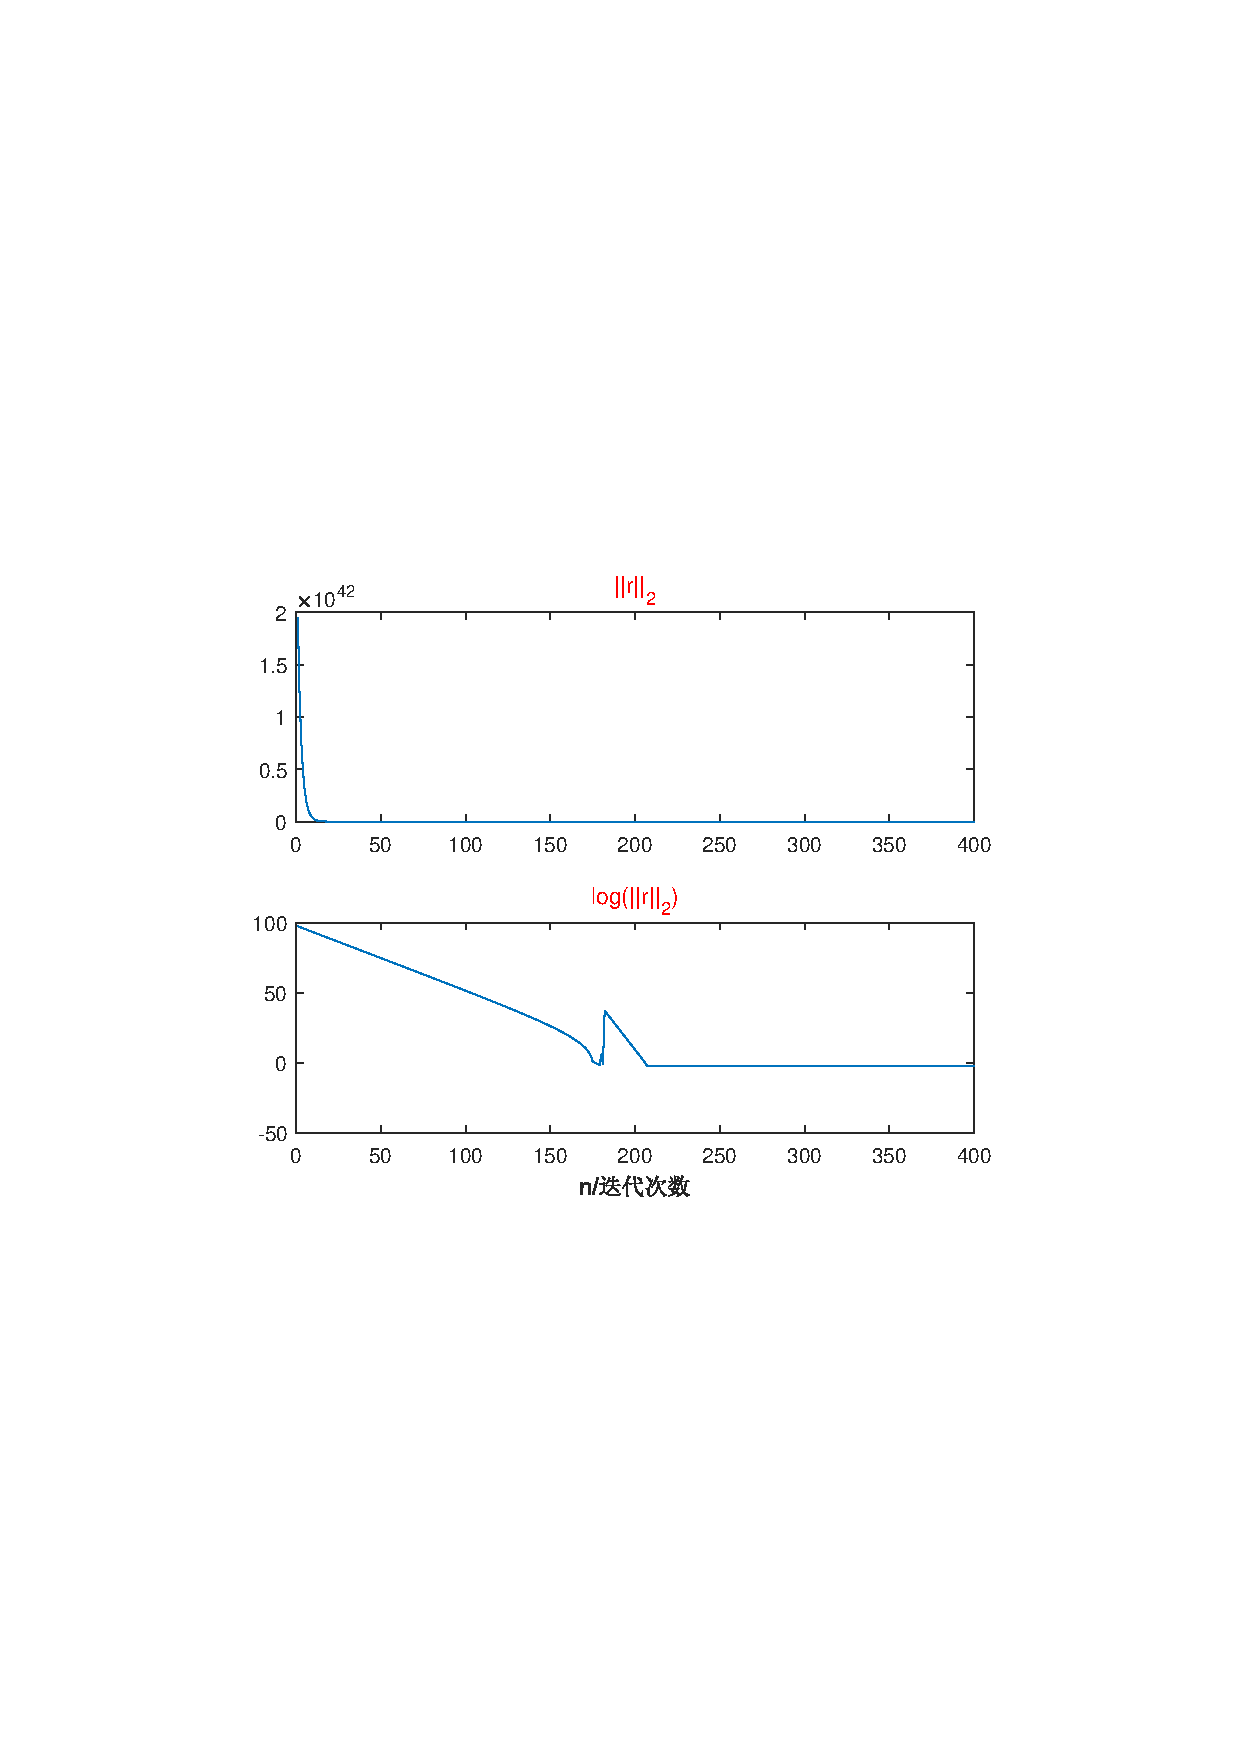
\includegraphics[width=10.5cm]{fig/6_3.pdf}
\caption{不带线搜索的GN法}
\end{figure}

\begin{figure}[H]
\centering
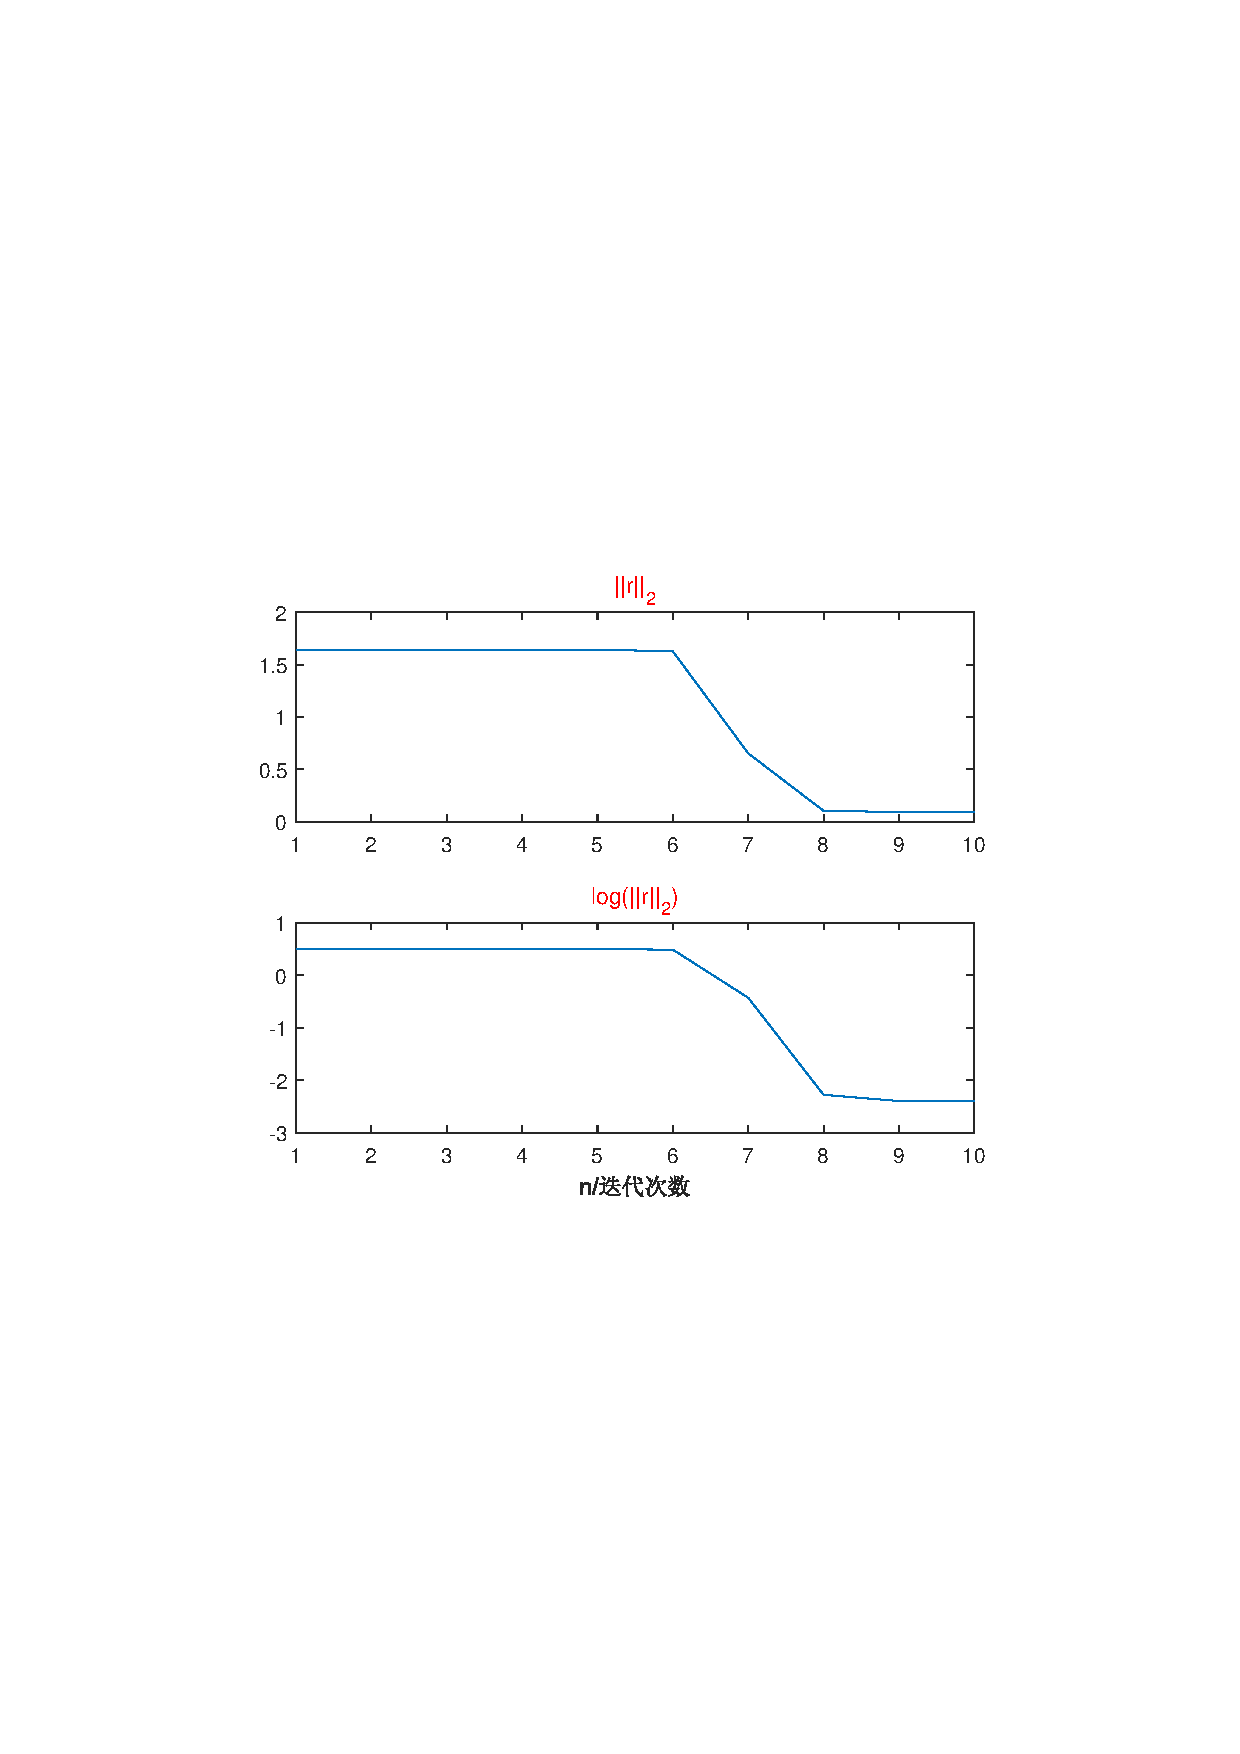
\includegraphics[width=12cm]{fig/6_4.pdf}
\caption{带线搜索的GN法}
\end{figure}

此外为了探查所得解与最优解之间的差异,我又调用了MATLAB优化工具箱中的lsqnonlin函数进行拟合,将两者进行比较,比较结果如下:

\begin{table}[H]
\centering
\caption{结果比较}
	\begin{tabular}{cccc}
	\toprule
	{}&带线搜索&不带线搜索&工具箱拟合\\
	\midrule
	stv&	0.0373	&0.0387&0.0267\\
	$x_1$&	3.3233e-04	&0.3252&-0.0096\\
	$x_2$&351.6673		&-6.8564e+03&-1.9017e+04\\
	\bottomrule
	\end{tabular}
\end{table}

\begin{figure}[H]
\centering
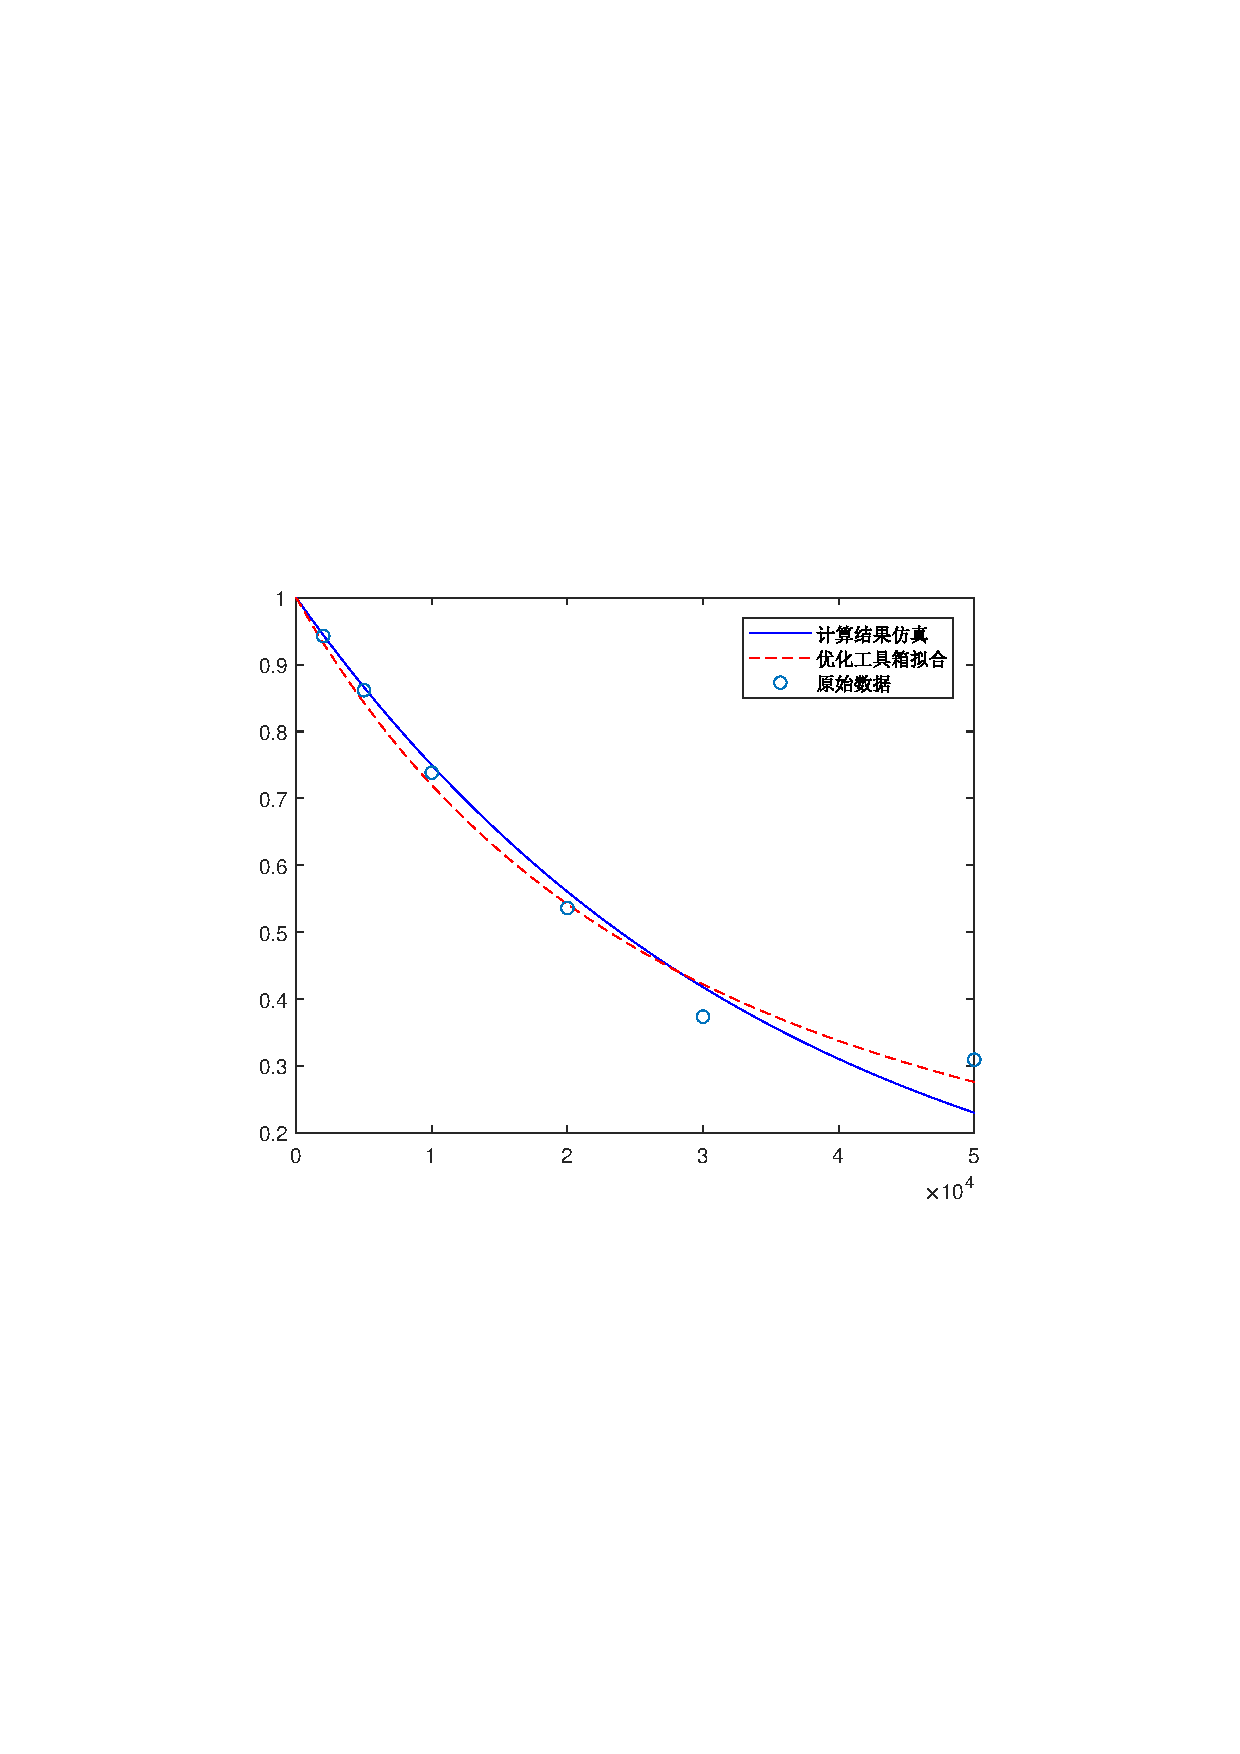
\includegraphics[width=9.8cm]{fig/6_5.pdf}
\caption{不带线搜索的GN法}
\end{figure}

\begin{figure}[H]
\centering
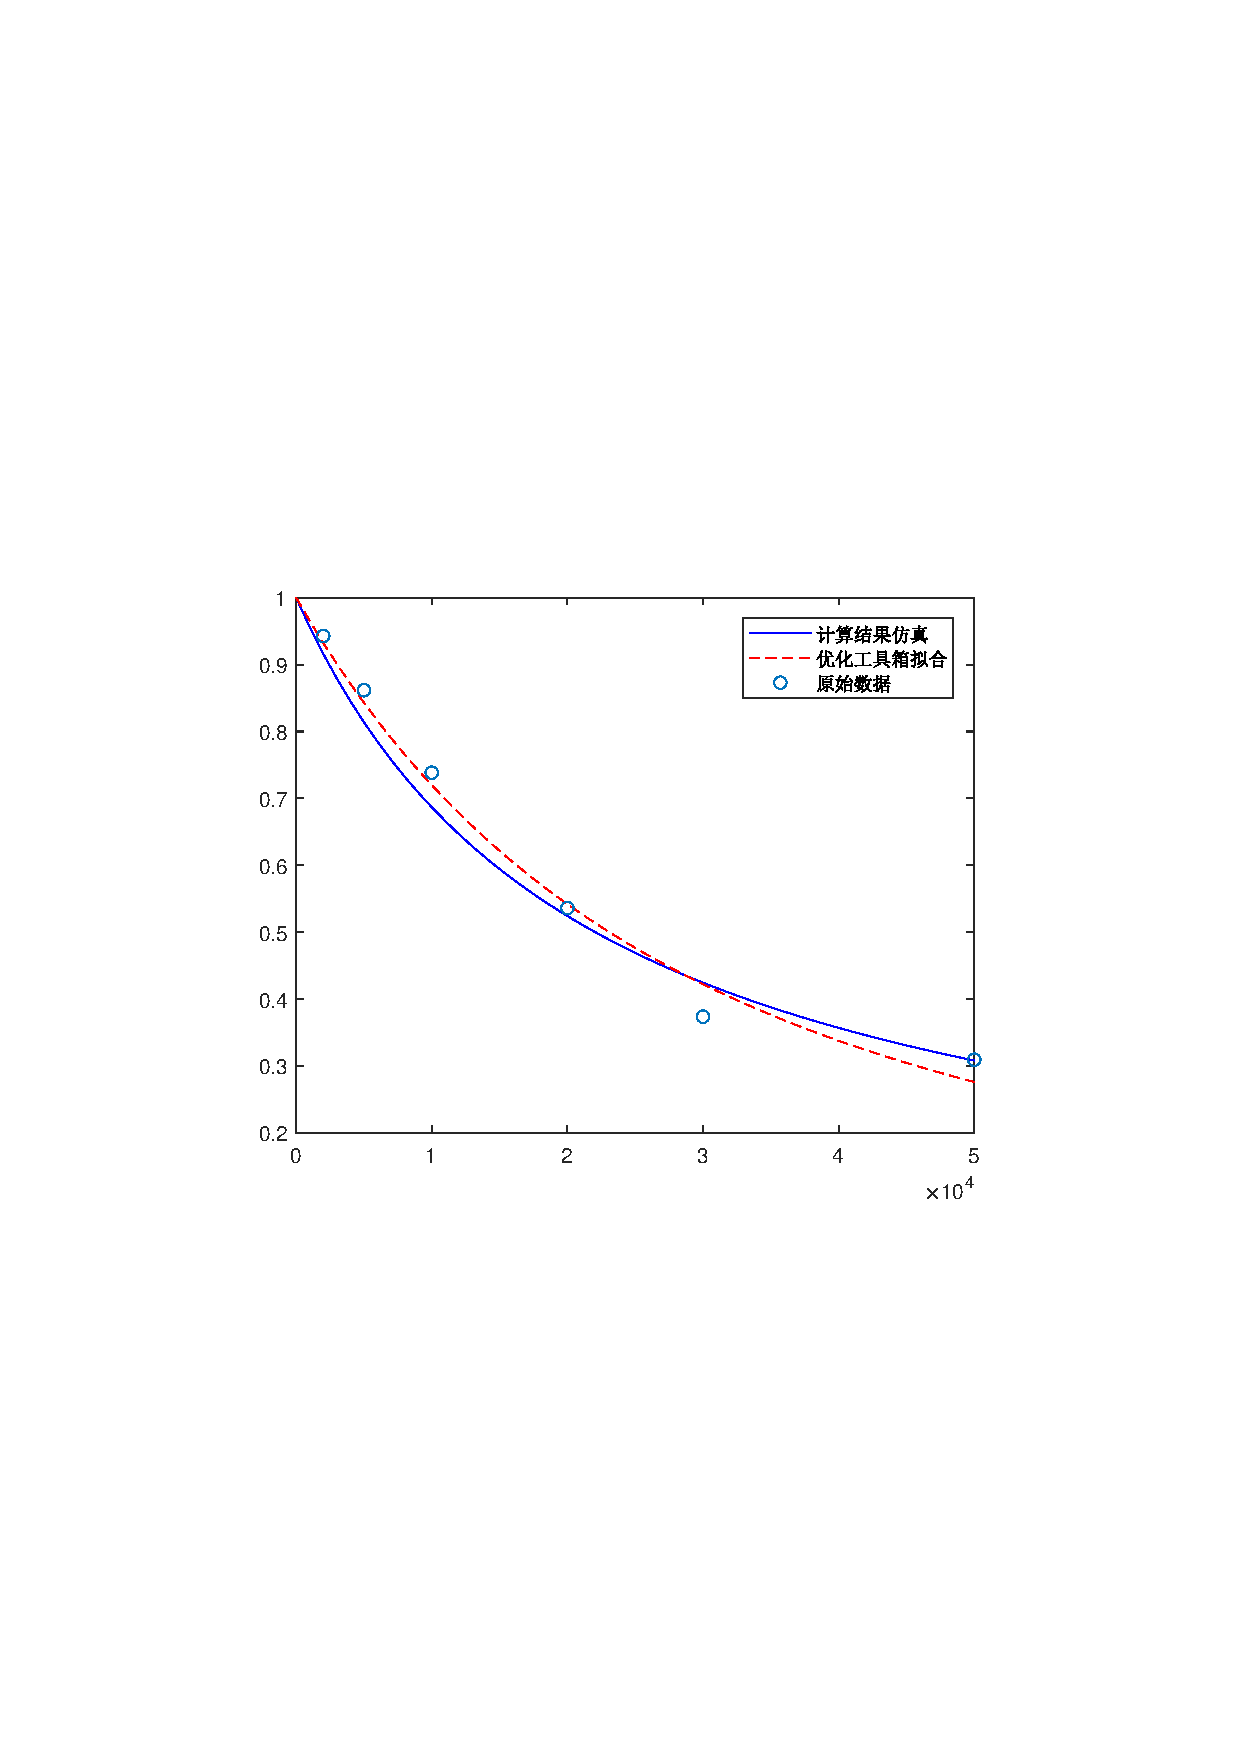
\includegraphics[width=9.8cm]{fig/6_6.pdf}
\caption{带线搜索的GN法}
\end{figure}

\subsection{总结分析}
首先,我们可以看出,在未使用Armijo线搜索时,程序花了约250步才迭代收敛,观察残差下降趋势,发现中间有一个较大的波动,将那个波动点提出出来,结果为$\bm{y}=$(1.897e-06,\ 11.541),越过这个点后误差函数明显增加了一截,然后迭代时继续下降。虽然最后也得到了误差较小的结果,但与全局极小点相去甚远。

而带了线搜索的GN法,只画了不到10步即收敛到了极小点,而且精度相当高,与全局极小的也很接近,可见带线搜索的GN法效果非常理想。

虽然三个结果互不相同,且差异不小,但由前面的拟合曲线可以看出,三者对原始数据都拟合得很不错。

\begin{table}[H]
\centering
\caption{拟合结果比较}
	\begin{tabular}{cccc}
	\toprule
	{}&带线搜索&不带线搜索&工具箱拟合\\
	\midrule
	$\bm{y}$&(-4.743e-05,\ 0.032)&(9.450e-07,\ 31.328)&	(-1.710e-05,\ -1.081)\\
	$\|\bm{r}\|_2$&	0.0915	&0.0947&0.0654\\
	\bottomrule
	\end{tabular}
\end{table}


我将误差函数曲面的图像画出来观察:


\begin{figure}[H]
\centering
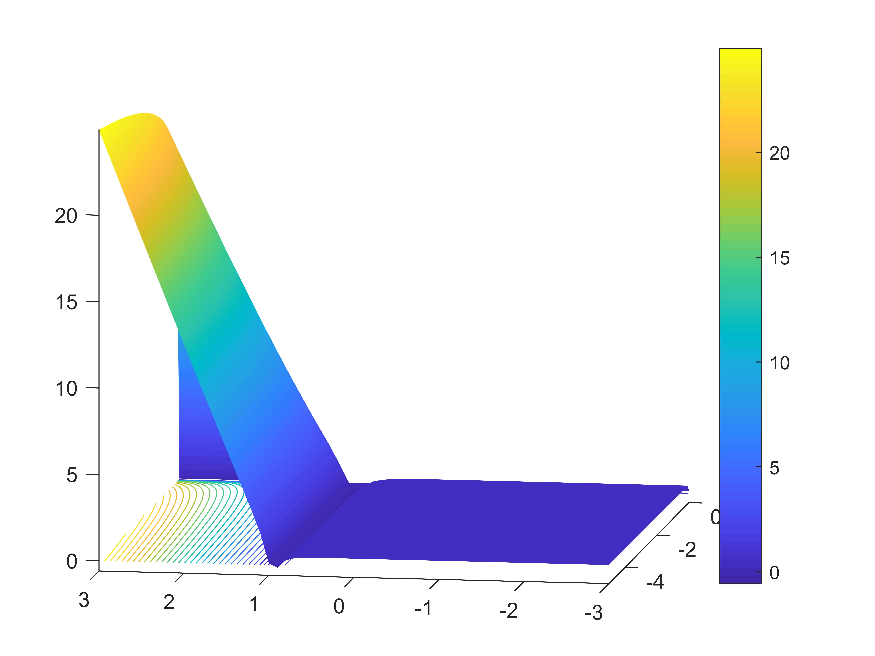
\includegraphics[width=9cm]{fig/6_1.pdf}
\end{figure}

可见在$y_2=1$附近有一条“沟”,全局极小点可能就处在上面,让我们将其放大并进行取对数操作观察:

\begin{figure}[H]
\centering
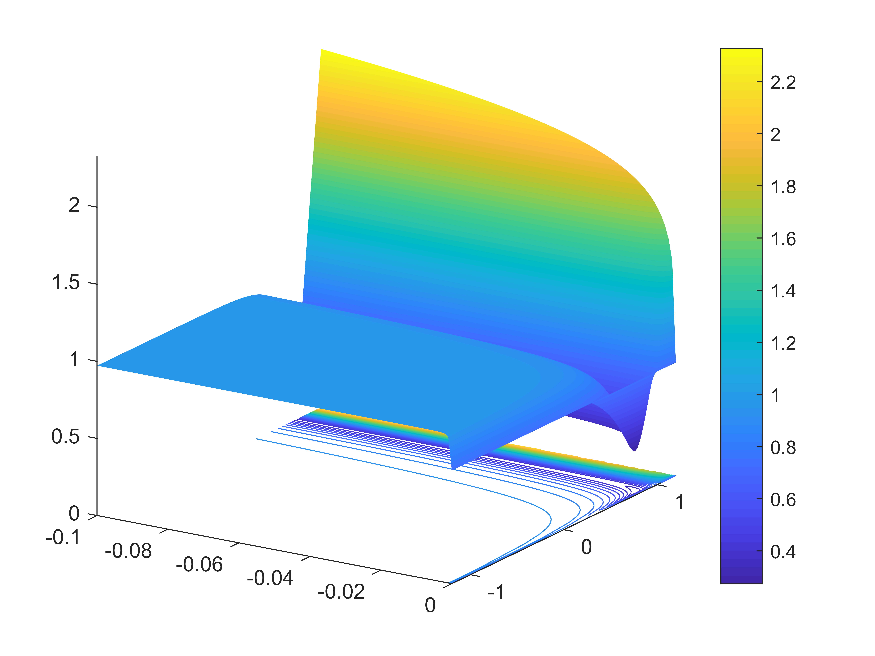
\includegraphics[width=10.5cm]{fig/6_7.pdf}
\end{figure}

\begin{figure}[H]
\centering
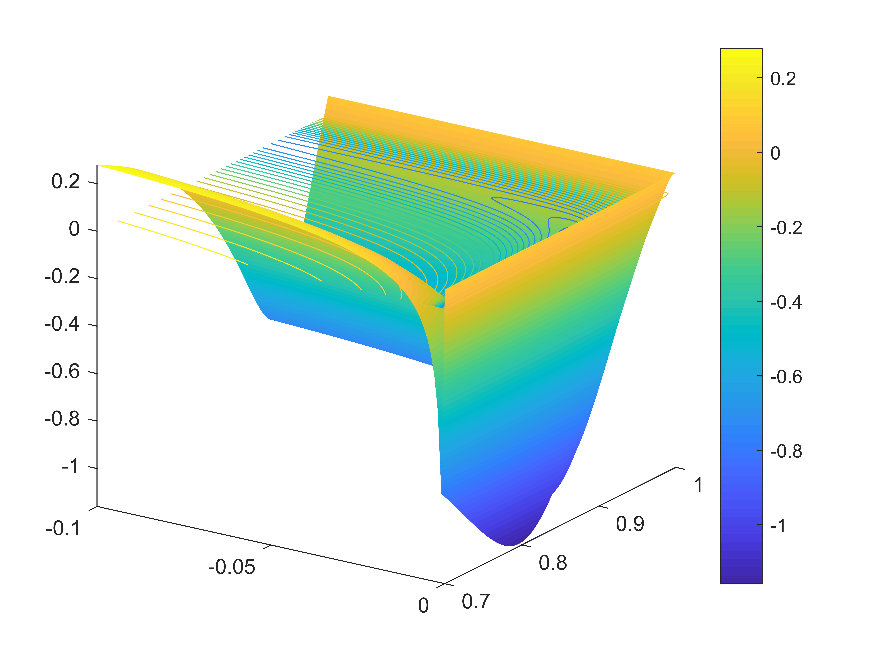
\includegraphics[width=10.5cm]{fig/6_2.pdf}
\end{figure}

然后发现从图上观察到的最小点为(-0.001,0.794),而将该点代入计算得残差为0.3146,比之前求的几个点误差都要大,初步揣测可能是MATLAB绘图精度问题,于是提高了精度,绘制出图像如下:

\begin{figure}[H]
\centering
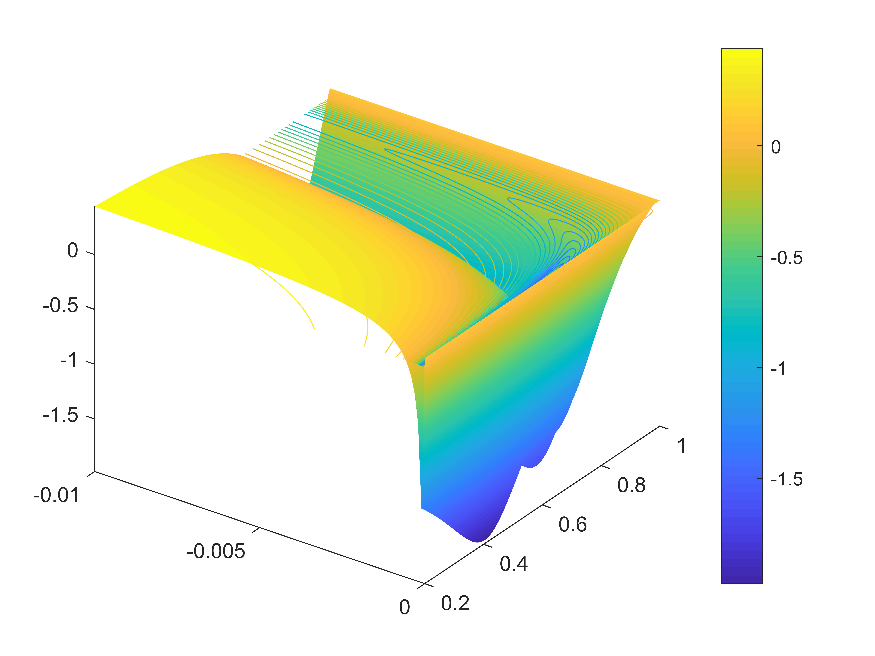
\includegraphics[width=12cm]{fig/6_8.pdf}
\end{figure}

此时观察图像,发现与之前的图像有不小的差别,沿着$y_1=0$这条线向下多出了几个低峰,取其中最低点的函数值为0.1383,仍然未达到我们计算的全局极小点,那么猜测沿着这条线向下,应该会继续多出几个越来越低的低峰,一直蔓延到真正的全局极小点,但是由于精度原因MATLAB无法完全绘制出来,足可见该函数之病态,因此我们的程序对参数的敏感性不是没有原因的。之前跑程序得出各种奇怪的结果,让我还一度以为程序出了问题。

此外,虽然此题中的$\bm{r}_i(\bm{x})$很小,但终究还是有一定误差,我猜测这就可能是为什么加了线搜索的GN法依旧没能迭代到最优点的原因吧。



